
% This LaTeX was auto-generated from MATLAB code.
% To make changes, update the MATLAB code and republish this document.

\documentclass{article}
\usepackage{graphicx}
\usepackage{color}

\sloppy
\definecolor{lightgray}{gray}{0.5}
\setlength{\parindent}{0pt}

\begin{document}

    
    \begin{verbatim}
function thirdTask
% Задаване на параметри
a = 1; b = 4; % граници на интервала
alpha = -0.3; %x(a)=alpha
beta = 0.4; % x(b)=beta
n = 100; % брой точки на дискретизация
h = (b-a)/(n+1); % стъпка на дискретизация
t=a:h:b;
% Дефиниране на матрицата на коефициентите и вектора на дясната страна
A = zeros(n,n);
f = zeros(n,1);
for i = 1:n
    if i ~= 1
        A(i,i-1) = h/(2*t(i)) - 1;
    end
    A(i,i) = 2 - (16*h^2)/(t(i)^2);
    if i ~= n
        A(i,i+1) = -h/(2*t(i)) - 1;
    end
    f(i) = -h^2*sin(1/t(i)^2);
end
% Прилагане на граничните условия
A(1,:) = 0; A(1,1) = 1;
A(n,:) = 0; A(n,n) = 1;
f(1) = f(1) - alpha*(h/(2*t(1)) - 1);
f(n) = f(n) - beta*(-h/(2*t(n)) - 1);
% Решаване на системата
x = A\f;
% Визуализация на решението
xx=[alpha;x;beta];
figure(4),plot(t,xx);
xlabel('t');
ylabel('x(t)');
title('Решение по метода на крайните приближения');
end
\end{verbatim}

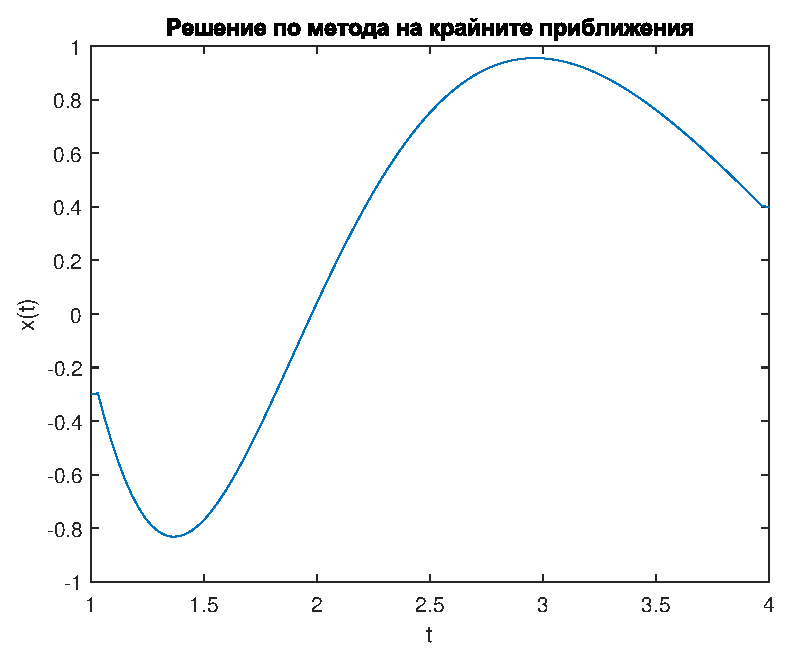
\includegraphics [width=4in]{thirdTask_01.eps}



\end{document}

